\section{Fonctions d'analyse}

	L'analyse détaillée d'ADtool a permis de mieux nous rendre compte des fonctionnalités d'analyse qui lui font défaut. Plutôt qu'implémenter ces dernières directement dans ADTool, nous avons fait le choix de créer un nouveau logiciel nommé \glasir\ qui utilisera cet éditeur d'arbres. Deux raisons nous ont poussé à prendre cette décision. La première est de séparer l'analyse et l'édition des ADTrees, afin d'avoir des logiciels dédiés à leur tâche. De plus, cette solution nous permet d'utiliser des technologies différentes de celles d'ADTool, enrichissant ainsi notre formation.  \glasir{} se chargera de la partie \textit{analyse}, et ADTool de la partie \textit{édition des arbres} sous forme de sous-fenêtre de \glasir{}. On peut voir sur la {\sc Figure} \ref{fig:architecture_Glasir} l'intégration d'ADTool dans l'architecture de \glasir{}. Nous avons choisi d'implémenter trois fonctionnalités principales, qui nous semblent répondre le mieux aux besoins d'un expert en sécurité.

		\begin{figure}[h!]
			\centering
				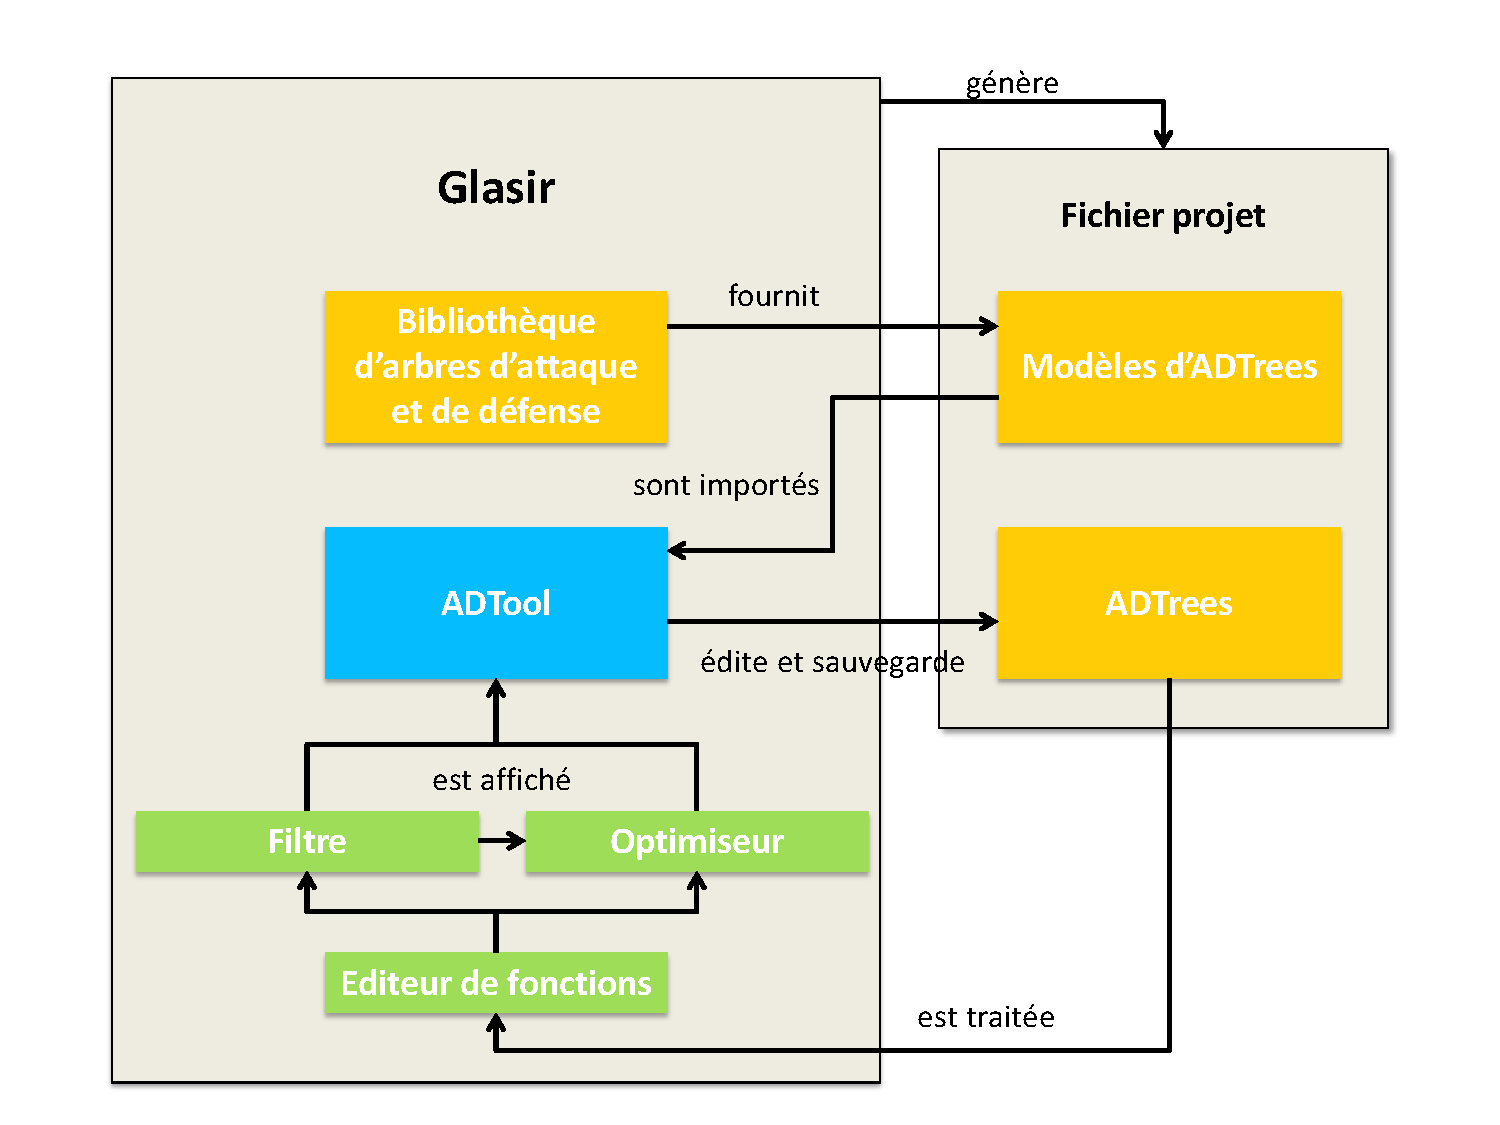
\includegraphics[width=0.6\textwidth]{figure/archiGlasir.pdf}
			\caption{Architecture du logiciel \glasir.}
			\label{fig:architecture_Glasir}
		\end{figure}

		\subsection{Optimiseur}
		\label{subsection:optimiseur}
		Une fois que l'expert a obtenu son arbre complet (qui peut se composer de plusieurs milliers de nœuds), il ne peut pas facilement identifier le chemin optimal selon un paramètre donné. Il s'agit en effet d'un travail manuel, relativement fastidieux, qui doit être recommencé à chaque modification de l'arbre.
		
		Pourtant, la méthode utilisée est systématique. Nous pouvons donc l'automatiser dans notre logiciel. Pouvoir identifier automatiquement le chemin optimal ferait gagner beaucoup de temps à l'utilisateur, et permettrait aussi de limiter les risques d'erreurs.

		Les entrées de l'optimiseur seraient donc celles-ci :
		\begin{itemize}
			\item Un arbre provenant du projet ;
			\item Le paramètre à prendre en compte ;
			\item Le critère ($min$ ou $max$).
		\end{itemize}

		Nous obtiendrons en sortie un nouvel arbre (qui sera un sous ensemble de l'arbre d'entrée), contenant le chemin optimal. 
		L'utilisateur pourra ensuite le traiter comme un tout nouvel arbre, en fonction de son besoin.
		
		Prenons en exemple l'arbre de la {\sc Figure} \ref{fig:pre_optimiseur}. Si on veut trouver un chemin optimal avec le paramètre \og coût \fg, et en critère la fonction $min$, on obtiendra l'arbre de la {\sc Figure} \ref{fig:arbre_post_opti}.
		
	\begin{landscape}
        \begin{figure}
            % \centering
            \includegraphics[height=0.82\textwidth]{figure/pre_optimiseur.pdf}
            \caption{Toto va a la plage.}
            \label{fig:pre_optimiseur}
        \end{figure}
    	\end{landscape}		
		
		\begin{figure}[h!]
			\centering
				\includegraphics[width=0.35\textwidth]{figure/post_optimiseur.pdf}
			\caption{L'attaque optimale est ainsi facilement lisible.}
			\label{fig:arbre_post_opti}
		\end{figure}
		
		
    
		
		
		Nous allons maintenant détailler l'algorithme qui parcourra l'arbre à la recherche du meilleur chemin. Il s'agira d'une fonction récursive.

		\begin{algorithm}[h!]
		\caption{opti}
		\begin{algorithmic}
			\STATE $l_fils \leftarrow fils(racine)$
			\IF{$vide(l_fils)$}
				\RETURN
			\ENDIF
			\IF{$mode(racine) == ou$}
				\STATE $v \leftarrow param(l_fils[0])$
				\FOR{$n in l_fils[1:]$}
					\STATE $v \leftarrow crit(v, param(n))$
				\ENDFOR
				\FOR{$n in l_fils$}
					\IF{$not defense(n) and param(n) != v$}
						\STATE delete(n) // will delete subtrees as well
					\ENDIF
				\ENDFOR
			\ENDIF
			\FOR{$n in fils(racine)$}
				\STATE $opti(n, param, crit)$
			\ENDFOR

		\end{algorithmic}
		\end{algorithm}

		L'algorithme modifiera l'arbre en l'état (c'est pour cela que nous le ferons travailler sur une copie de l'arbre).
		\begin{itemize}
			\item \verb|racine| correspond au nœud à partir duquel nous élaguerons l'arbre.
			\item \verb|param| est une fonction renvoyant une valeur pour un nœud donné.
			\item \verb|crit| est une fonction prenant en paramètre deux valeurs et renvoie la valeur à \og garder \fg.
			\item \verb|fils| est une fonction renvoyant une liste de nœuds, correspondants aux fils du nœud passé en paramètre.
		\end{itemize}

		Ainsi, pour lancer l'optimisation, nous appellerons notre fonction \verb|opti| avec la racine de l'arbre en paramètre.
		La fonction est récursive et la complexité, dans la pire des configurations, est linéaire.

	\subsection{Filtre}
	\label{subsection:filtre} 
		Souvent, l'expert en sécurité va chercher à se défendre contre un attaquant précis. Dans ce cas, il va chercher à identifier les ressources dont l'attaquant dispose (temps, argent, etc.), pour ne conserver que les chemins de l'arbre empruntables par l'attaquant.

		Nous allons donc implémenter une fonctionnalité permettant de répondre à ce besoin, que nous appellerons \textit{filtre}. L'expert devra définir un critère selon lequel effectuer le filtrage, puis choisir un intervalle dans lequel les valeurs du paramètre devront se situer.

		Les entrées de la fonction de filtrage seront les suivantes :
		\begin{itemize}
			\item l'arbre à filtrer ;
			\item les valuations de l'arbre servant de critères pour le filtrage ;
			\item les intervalles de sélection sur les différentes valuations.
		\end{itemize}
		
		Il sera possible de filtrer l'arbre avec plusieurs paramètres simultanément.
		L'arbre retourné par la fonction de filtrage sera une copie élaguée de l'arbre original. Seuls les chemins respectant les intervalles de filtrage seront conservés.

		Par exemple, en appliquant un filtre sur l'intervalle $[0, 500]$ et sur la valuation \og coût \fg à l'arbre de la {\sc Figure} \ref{fig:arbre_post_opti}, on obtient l'arbre de la {\sc Figure} \ref{fig:arbre_post_filtre}.

		\begin{figure}[!h]
			\begin{center}
				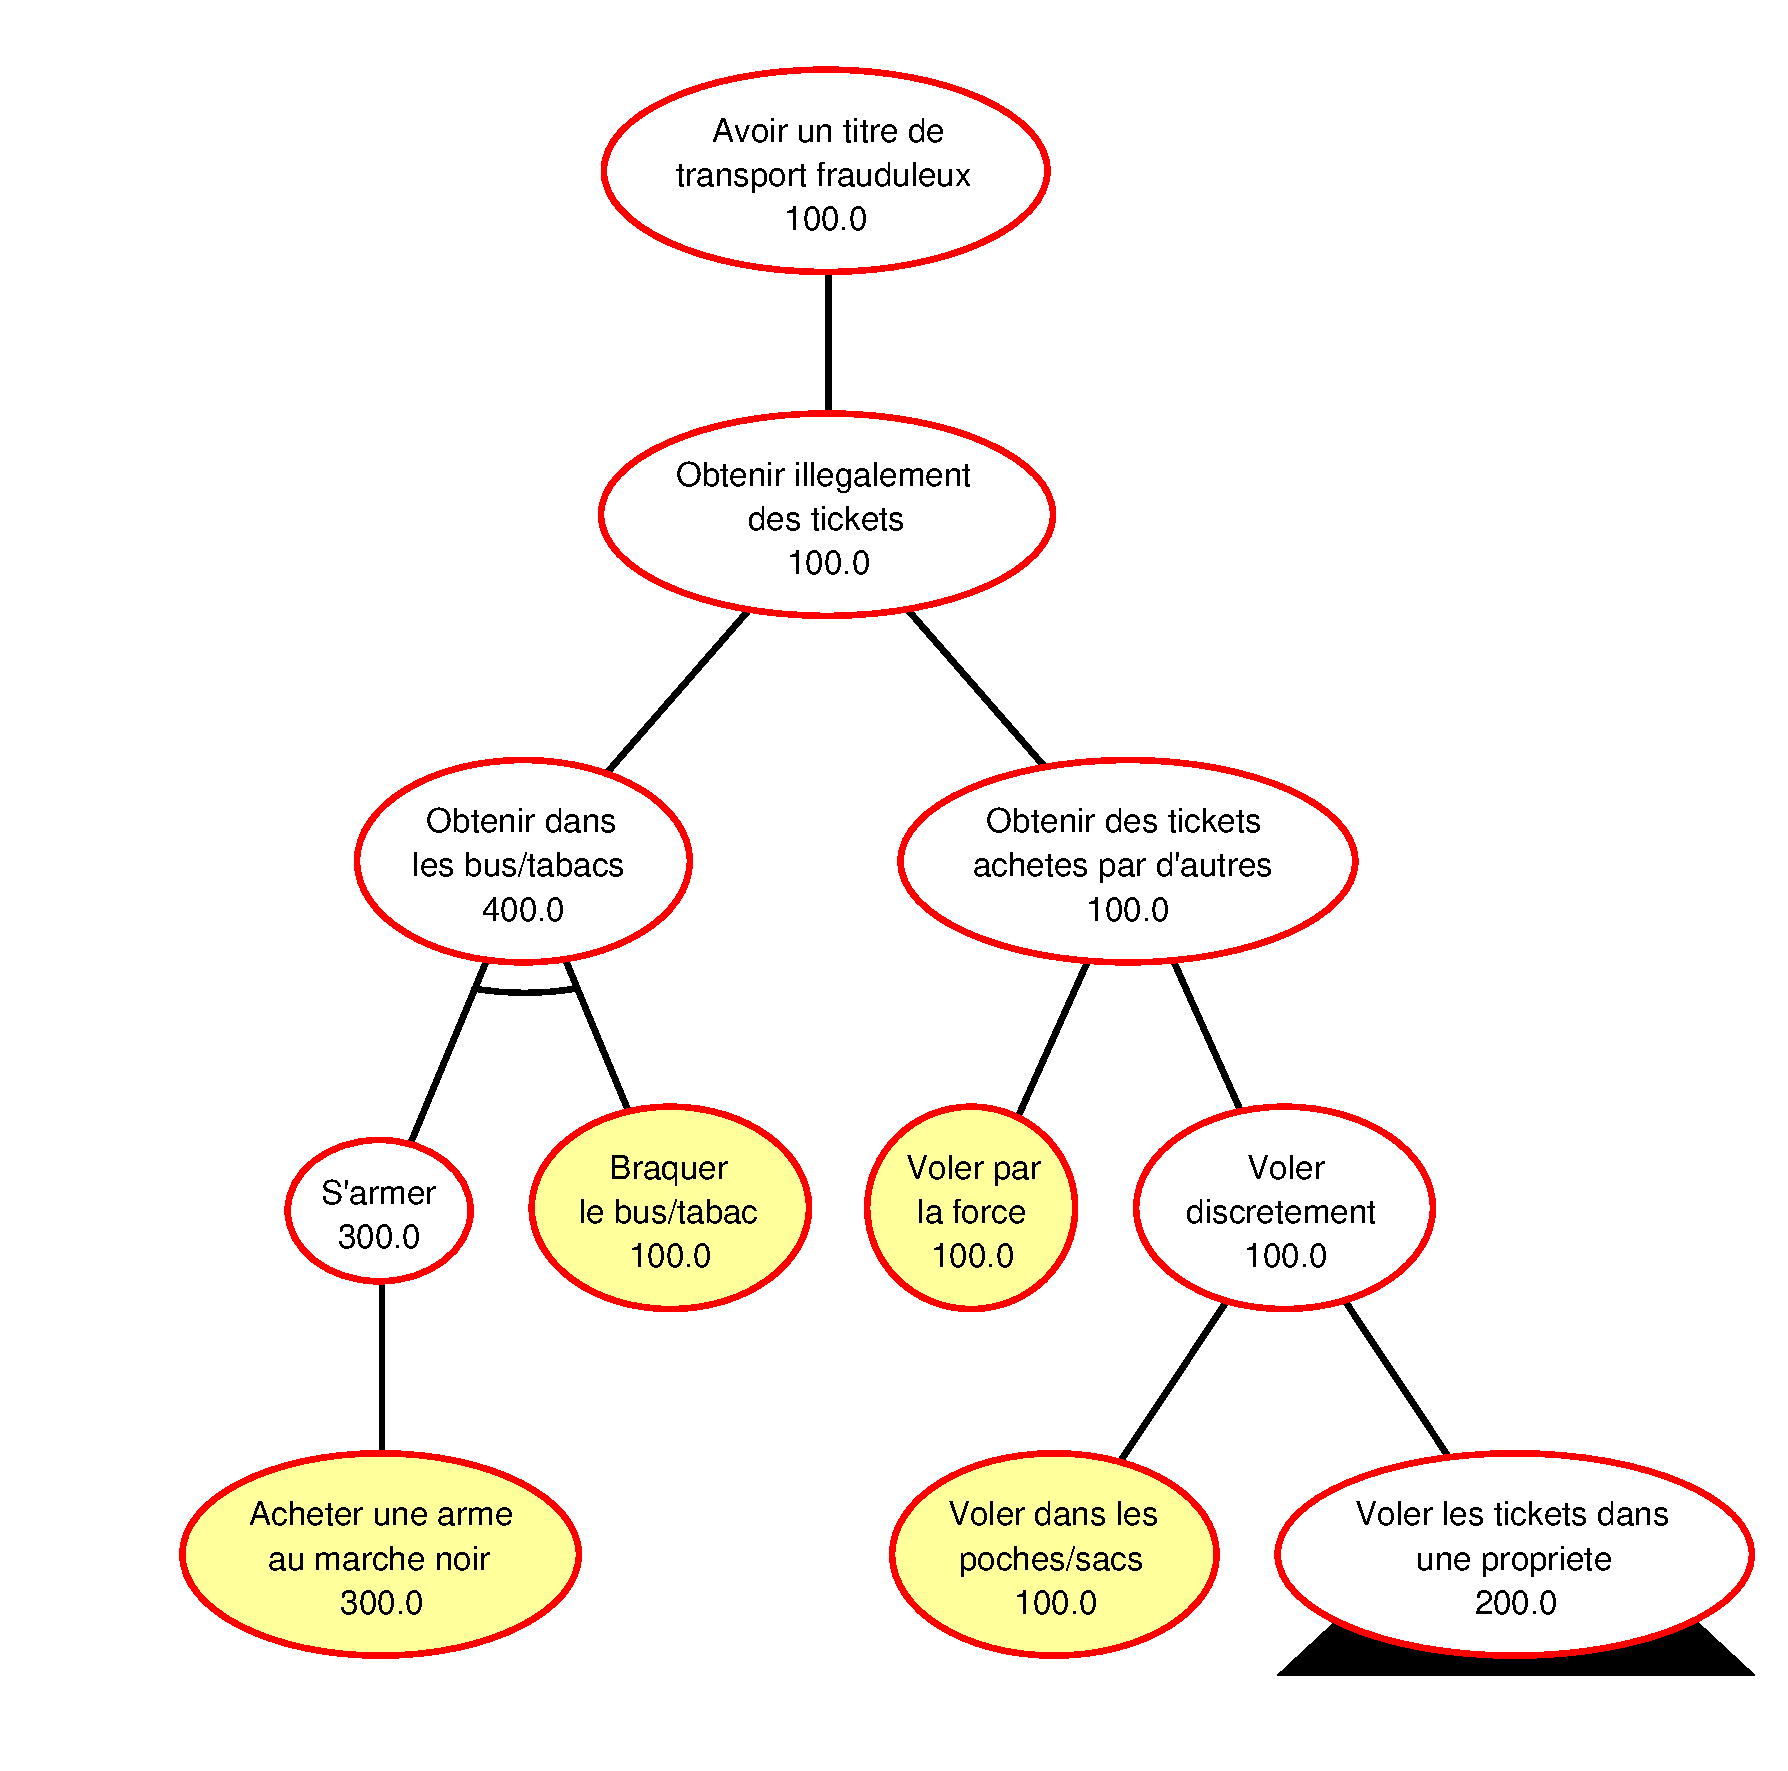
\includegraphics[width=0.75\textwidth]{figure/post_filtre.pdf}
			\end{center}
			\caption{Filtre selon le coût pour l'attaquant}
			\label{fig:arbre_post_filtre}
		\end{figure}
		On constate que l'arbre élagué par le filtre a été considérablement réduit. L'arbre exemple étant de taille très réduite comparé aux modélisations de systèmes réels, on comprend bien l'utilité de cette fonctionnalité pour l'expert.

		D'un point de vue technique, il nous semble intéressant d'aborder la manière dont l'arbre sera élagué par le filtre.
		L'algorithme de filtrage suivra ce modèle :

		\begin{algorithm}[h!]
			\caption{filtre}
		\begin{algorithmic}
			\STATE{filtre(racine, rules)}
				\FOR{r in rules}
					\IF{not r(racine)}
						\STATE delete(racine AND subtrees)
						\RETURN
					\ENDIF
				\ENDFOR
				\FOR{n in fils(racine)}
					\STATE filtre(n, rules)
				\ENDFOR

		\end{algorithmic}
		\end{algorithm}

		\begin{itemize}
		 \item \verb|racine| est le point de départ de l'algorithme.
		 \item \verb|rules| est l'ensemble des règles de filtrage (valuation et intervalle).
		\end{itemize}
	
		Le principe de l'algorithme est récursif.
		Le nombre d'appels sera, au pire, linéaire avec le nombre de nœuds de l'arbre.
		La complexité algorithmique est donc acceptable.

		\subsection{Paramètres de synthèse}
		\label{subsection:synthese} 

			L'utilisateur est actuellement cantonné aux paramètres présentés précédemment dans la section 2, et ne peut pas en créer d'autres, ce qui limite ses possibilités d'analyse et d'interprétation. En effet, les paramètres déjà existants ne sont pas les seuls pouvant intéresser un expert en sécurité. Nous souhaitons donc rendre possible la création de nouveaux paramètres, à partir de ceux déjà disponibles et des fonctions mathématiques de base (division, multiplication, min, max, etc). Ces nouvelles valuations pourront ensuite être appliquées à n'importe quel arbre, de la même manière que les paramètres de base. Elles pourront ainsi être utilisées pour analyser les arbres selon de nouveaux critères, et si besoin pour les élaguer à l'aide du filtre que nous allons implémenter.\\

			Cette nouvelle fonctionnalité, appelée \emph{éditeur de paramètres}, prendrait donc en entrée les éléments suivants :
			\begin{itemize}
				\item un arbre provenant du projet courant; % quel projet ?
				\item les paramètres intervenant dans la synthèse ;
				\item les opérations mathématiques appliquées ;
				\item le nom du paramètre de synthèse généré.
			\end{itemize}


			\paragraph{}
			Par exemple, dans notre arbre illustratif disponible en Annexe de ce rapport, nous pouvons voir que les deux sous-arbres « Obtenir illégalement des tickets » (sous-arbre A) et « Falsifier des tickets » (sous-arbre B) permettent d'atteindre l'objectif final. Il est actuellement possible de les valuer par treize paramètres, nous n'en garderons ici que deux pour simplifier : le coût minimal et la probabilité de succès.\\ % figure ?

			On constate rapidement que choisir A implique un coût de réalisation moindre pour l'attaquant puisqu'il nécessite peu de matériel. Cependant, un vol est toujours risqué, et les chances de se faire arrêter sont élevées. Opter pour le sous-arbre B, bien que plus cher à réaliser, permet de limiter ces risques : la probabilité de succès est donc plus forte. On voit donc que ces deux paramètres, qui ne sont pas liés, peuvent être tous les deux utiles à l'utilisateur et entraîner une interprétation très différente. C'est pourquoi il serait intéressant de pouvoir les combiner, grâce à notre éditeur de paramètres, afin de les prendre en compte tous les deux. C'est ensuite à l'utilisateur de juger des liens qu'il désire instaurer entre les paramètres : fonctions mathématiques, coefficients, etc. Par exemple, si l'on décide d'appeler le nouveau paramètre « result », et que l'on estime qu'il s'agit du coût auquel on ajoute la probabilité de succès multipliée par deux, on obtient la synthèse suivante : \[ result = (minimal\_cost) + 2 \times (probability\_of\_success).\]
